\documentclass{standalone}
\usepackage{graphicx}	
\usepackage{amssymb, amsmath, amsthm}
\usepackage{color}

\usepackage{tikz}
\usetikzlibrary{intersections, backgrounds, arrows.meta}

\definecolor{light}{RGB}{220, 188, 188}
\definecolor{mid}{RGB}{185, 124, 124}
\definecolor{dark}{RGB}{143, 39, 39}
\definecolor{highlight}{RGB}{180, 31, 180}
\definecolor{gray10}{gray}{0.1}
\definecolor{gray20}{gray}{0.2}
\definecolor{gray30}{gray}{0.3}
\definecolor{gray40}{gray}{0.4}
\definecolor{gray60}{gray}{0.6}
\definecolor{gray70}{gray}{0.7}
\definecolor{gray80}{gray}{0.8}
\definecolor{gray90}{gray}{0.9}
\definecolor{gray95}{gray}{0.95}

\begin{document}

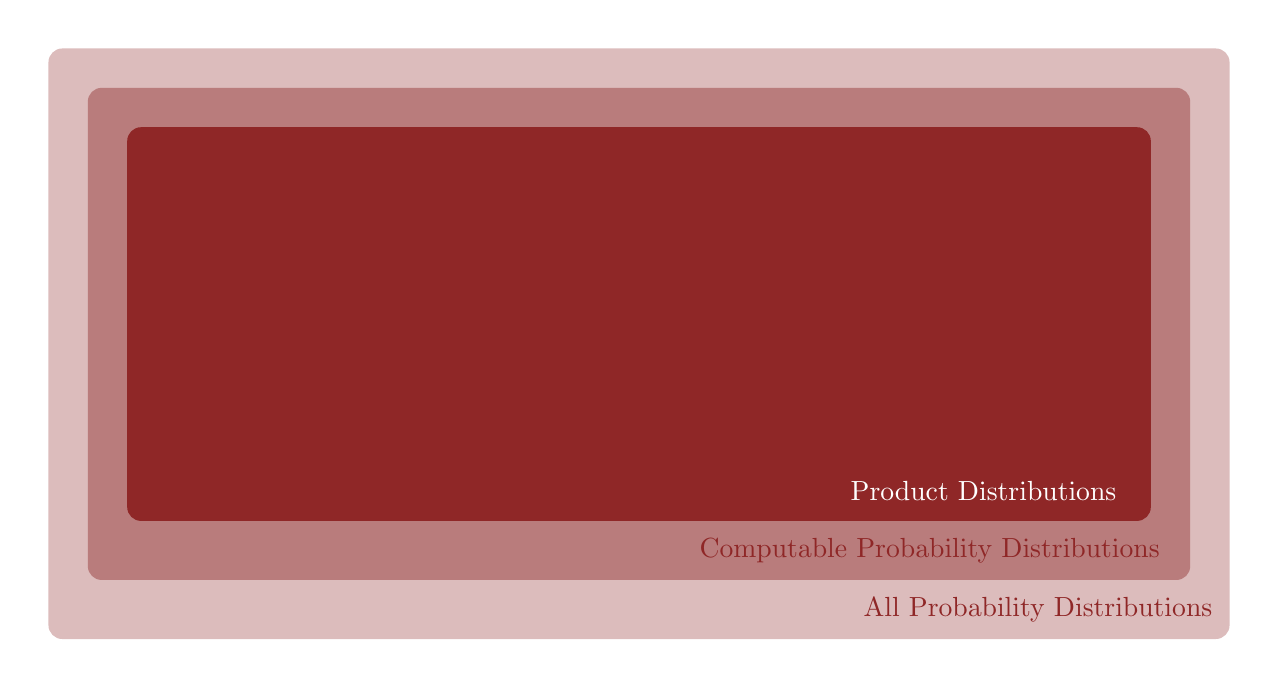
\begin{tikzpicture}[scale=0.25, thick]
  \draw[white] (-31, -16) rectangle (31, 16);
  
  \fill[rounded corners=5pt, light] (-30, -15) rectangle +(60, 30);
  \node[text=dark, align=center] at (20.5, -13.5) { All Probability Distributions };

  \fill[rounded corners=5pt, mid] (-28, -12) rectangle +(56, 25);
  \node[text=dark, align=center] at (15, -10.5) { Computable Probability Distributions };

  \fill[rounded corners=5pt, dark] (-26, -9) rectangle +(52, 20);
  \node[text=white, align=center] at (17.5, -7.5) { Product Distributions};
  
\end{tikzpicture}

\end{document}  